\documentclass[a4paper, 11, margin=2cm]{article}
\usepackage{graphicx}
\usepackage{lineno}
\usepackage{float} 
\usepackage{authblk} 
\usepackage{natbib}
\usepackage{caption}  
\usepackage{subcaption}
\usepackage{setspace}
\usepackage[scaled]{helvet}

\onehalfspacing
\captionsetup[figure]{font=small}
\captionsetup[table]{font=small}

\title{\LARGE {Assessing the functional composition and diversity of plants in the Pound Hill by seed traits} \\
 \vspace*{20mm}}

\author{\textbf{Shiyuan Huang} \\Email: shiyuan.huang22@imperial.ac.uk \vspace*{4mm}}

\date{August 2023 \vspace*{30mm}}

\affil{\textbf{Imperial College London} \vspace*{10mm}}

\begin{document}
    
    \begin{titlepage}
      \maketitle
      
    \begin{center}
      \textbf{A thesis submitted in partial fulfilment of the requirements for the degree of Master of Science at Imperial College London \\ \vspace*{2mm}
      Submitted for the MSc in Computational Methods in Ecology and Evolution} 

    \end{center}
    
    \end{titlepage}

    
    \pagebreak

    \newpage
    \thispagestyle{empty} 
    \mbox{} 

    \begin{center}
      \textbf{Declaration}
    \end{center}
    
  
    \noindent{\\ I declare that the raw data was provided by my supervisor Josh Hodge from Imperial College London. \\ \\ I declare that I was responsible for all the data processing. \\ \\ I declare that no mathematical models were developed by me or my supervisor. \\ \\ My supervisor Josh Hodge provided me with technical Q\&A support and feedback in developing the analyses presented. \\ \\}


    
    \pagebreak

    \section{Abstract}

    Plant traits are gradually capturing the interest of ecologists. Exploring how to study plant communities based on seed traits holds significant potential, and ecologists are accelerating research on trait-based abundance prediction models. This study aims to assess the effects of cultivation and soil disturbance timing on the functional composition and diversity of the Pound Hill plant community by seed traits. Additionally, the predictive capacity of the Fourth Corner model for species relative abundance is evaluated. By cultivating in March, May, and October each year, the functional traits of the Pound Hill plants exhibited variations. Seeds cultivated in March showed high germination rates and the highest germination temperature. Seeds from May cultivation exhibited the highest germination rate, along with the longest seed longevity and seedbank duration. October cultivation resulted in a larger seed mass. Furthermore, the March-cultivated community displayed higher functional divergence, indicating intense competition among functionally similar species. May-cultivated communities exhibited higher functional richness and evenness, implying more uniform resource utilization and stronger resistance to invaders. In contrast, October-cultivated communities showed lower functional evenness and divergence, suggesting reduced inter-species competition and lower resource utilization. These communities had simpler structures and weaker resistance to invaders. For the Fourth Corner model fitting, better predictions were achieved by including only the year and cultivation month as predictors. Incorporating more traits could enhance accuracy, but excessively adding variables to the model might decrease prediction precision. Notably, the Fourth Corner model with only site information as a predictor did not perform optimally. These findings demonstrate the impact of altering cultivation timing on functional composition and diversity of plant community. Using the Fourth Corner model for species relative abundance prediction is feasible, although the results are not the best.


    \section{Introduction}

    Seedling recruitment, which is dependent on seed germination and seedling survival, shapes plant communities. Community ecology is widely using trait-based techniques to address longstanding queries about species distribution and abundance along gradients \citep{zirbel2020trait}. The study of seed traits has been neglected to a large degree in explaining the presence and abundance of species \citep{rosbakh2022inferring}. Research on seed traits can improve the comprehension of the functional space of plant traits, as seed traits are usually not related to traits of mature plants such as leaf, and they are less plastic \citep{jimenez2016seed}. It is predicted that differences in the timing and intensity of disturbances will have an impact on the relative abundance of plant species and the composition of the seed bank since species vary in the ideal circumstances for germination. Cultivation in the autumn selects species that grow rapidly the following spring after experiencing severe winter weather. Cultivation in March favours the germination of vernalized seeds. Cultivation in May allows seedlings to grow in conditions that are frequently dry with a short growing season, favouring species that grow rapidly after frost \citep{crawley2004timing}. In general, seed regeneration is more susceptible to environmental changes such as temperature, salt, humidity, and oxygen than the growth of mature plants since germination is not only irreversible but also the most fragile stage of a plant's lifespan \citep{jimenez2016seed}. In order to incorporate regeneration traits into predictive models as well as ecological studies, it is essential to study how various seed traits shape community \citep{saatkamp2019research}.

    Functional traits and diversity might be an effective strategy to refine the research on the links between seed traits and plant communities. Seed traits capture a variety of morphological and physiological attributes of seeds. The distribution of trait values in communities can be mapped by various metrics of functional diversity \citep{lavorel2008assessing}. Choosing appropriate functional diversity metrics may assist us in comprehending and assessing the effects of the timing of cultivation and soil disturbance on species composition. Functional diversity can be described in terms of three different dimensions: richness, evenness, and divergence. Richness reflects how much total diversity is present in the species community; evenness reflects the regularity of the spatial distribution of the species' traits; and divergence reflects the variation in the distribution of species from their average position \citep{mammola2021concepts}.

    How to predict species abundance is one of the most interesting topics for ecologists, with how to use biological principles such as species traits to predict species abundance being a popular topic \citep{laughlin2012predictive}. Our goal is to select a model that can combine seed traits with environmental filters and species abundance for analysis. The problem of predicting the association between species traits and the environment by combining species abundance, species traits, and environmental variables is known as the fourth-corner problem, and a model of the fourth-corner problem can predict species abundance in new environments by quantifying the association between traits and the environment \citep{brown2014fourth}. Exploring various combinations of traits and environmental variables for better prediction will be a topic of interest as well.

    This study assessed the impact of cultivation and soil disturbance timing on the functional traits and diversity of the Pound Hill plant community. The variation in functional traits and diversity across different cultivation months were examined. Furthermore, the influence of different trait combinations on the predictive capacity of the Fourth Corner model for species relative abundance was evaluated. Our hypothesis was that variations in cultivation timing would result in variation in the functional trait composition of the Pound Hill plant community: the seedbank duration might exhibit changes consistent with seed longevity, while seed quality could be negatively correlated with seedbank duration \citep{crawley2004timing}. Longer seedbank duration might provide more germination opportunities. March cultivation might favor species with lower germination temperatures. In terms of community functional diversity, March cultivation could lead to reduced functional richness and increased divergence, while the cultivation in May might increase the functional richness. October cultivation might introduce dominant species and decrease functional evenness \citep{crawley2004timing}. For predictive models, an increased number of functionally representative traits might enhance the predictive performance of the Fourth Corner model.

    \section{Material and methods}
     
    \subsection{Data}
    
    The species data used in this research was obtained from the Pound Hill Disturbance Experiment, which was established in 1991 in an area of Silwood Park to maintain the conservation of arable weeds by annual cultivation in March, May, and October. This has transformed the original wheat land in the area into a mostly annual weed community. From 1987 to 2019, Silwood Park has had an average annual rainfall of 679mm with little seasonal variation. The mean hourly temperature is $ 10^\circ C $ with a July max of $ 23^\circ C $ and February min of $ 1.2^\circ C $. The experiment is located in Pound Hill field. It is situated on acidic, sandy soils of the Bagshot Series and is bounded by naturally regenerated alder woodland. This data can be accessed at https://www.imperial.ac.uk/silwood-park/research/silwood-lte/poundhill-disturbance. Here I chose PoundHillDist\_cover.csv for for sites and species abundance data, which consists of cover data for each plant species collected in 2014, 2016, 2017, 2019, 2020, and 2021. The environmental data that were to be used in this study included year, block, plot, and month. Three 36 * 8 m plots were cultivated in March, May, or October, each divided into four 36 * 36 m blocks (A to D). Afterwards, the three cultivation treatments were repeated four times. The month is the month of cultivation, the year indicates the year in which the data was collected, block represents the block containing each of the three cultivation treatments, and plot(1 - 12) represents each plot cultivated in each block. To obtain the relative abundance of species, the total abundance of each site was obtained by summing all the species in each site and then dividing the abundance of each species by the total abundance of the corresponding site to obtain the relative abundance.

    Trait data for each species at Pound Hill were obtained from the TRY Plant Trait Database (https://www.try-db.org/) for the following five traits: Seed dry mass, Seed germination rate, Seed (seedbank) longevity, Seed germination temperature, and seedbank duration. The trait data obtained from the TRY Plant Trait Database provided standardized trait value data (Trait values after unifying units for each trait). The standardized units for the five trait values are as follows: seed dry mass in $mg$, seed (seedbank) longevity in $years$, seedbank duration in $months$, seed germination rate in $\%$ and seed germination temperature in $ ^\circ C $. We would also refer to these five traits later as seedmass, longevity, seedbank duration, germination rate, and temperature, respectively.

    Seed dry mass is related to the dispersal distance of the seed, its ability to survive in the soil, and the likelihood of predation by herbivores. Larger seeds usually have higher nutrient stores, which may have a positive effect on germination and seedling survivability. Seed germination rate describes the competitive ability of seeds to germinate in extreme environments. This trait provides information on seed vigor and survivability and is important for the reproductive success and ecological adaptability of plants \citep{jimenez2016seed}. Seed (seedbank) longevity is the longevity of seeds after maturation or dispersal. A longer survival period gives plants a higher chance of surviving and reproducing, especially under unstable environmental conditions. Seed germination temperature helps us understand how well plants adapt to temperature changes and is related to the ability of seeds to adapt to climate, seasonal detection, and ecological niche width. Seedbank duration refers to the duration of time that seeds are stored in the soil. The seedbank duration is related to the life cycle and population dynamics of the plant and has important implications for the genetic diversity of seeds, population dispersal, and population stability \citep{jimenez2016seed}.

    \subsection{Imputation of missing data}

    Missing trait values were observed in few species: 5 missing values for longevity, 6 for germination rate, 14 for germination temperature, and 3 for seedbank duration. For missing trait values, a simple practice is to remove species with missing trait data and use only species with complete trait values. However, as this practice may lead to biased results, this approach is not recommended; a better approach is data imputation \citep{debastiani2021using}. First, I calculated the mean of each trait value for each species, accounted for the missing trait values, and filled in the missing traits with NA. Next, the method of inputation needed to be chosen. Random forests is a mechanical learning technique that can handle mixed types of data and allows for interaction and non-linear effects \citep{breiman2001random}. I decided to use MissForest with a phylogenetic tree to estimate the missing trait values in this research. The method was provided by a R package called funspace \citep{funspace}, and the phylogenetic tree was built using a function provided by another R package V.PhyloMaker2 \citep{V.PhyloMaker2}. To test whether adding phylogenetic information could improve the imputation of MissForest, I also compared the imputation results of MissForest with a phylogenetic tree with MissForest without a phylogenetic tree. Firstly, I filtered out the non-NA data from the original data and converted 20\% of this data into NA. Then I used MissForest and MissForest with a phylogenetic tree to impute these data, respectively. Finally, the Root Mean Squared Error(RMSE) values between the two imputations and the original data were calculated separately and compared. I performed 1000 different missing simulations on 20\% of the non-NA data and imputed these 1000 simulations with two MissForests. MissForest with a phylogenetic tree had smaller RMSE values than MissForest without a phylogenetic tree in 900 simulations, their means were 0.947 and 1.083, respectively. The results indicate that MissForest with a phylogenetic tree may have a better performance in imputation for our trait dataset. Therefore, I decided to use MissForest with a phylogenetic tree to impute the missing data.

    The Root Mean Square Error (RMSE) is a metric of the mean variation between the predicted and actual values of a statistical model. Mathematically, it represents the standard deviation of the residuals, which is the distance between the regression line and the data points. In other words, RMSE is used to assess the accuracy of model predictions, with smaller values indicating that the model predictions are closer to actual observations. And the formula for RMSE is:


      \begin{equation} RMSE = \sqrt{\frac{sum(pred - real)^2}{N}}  \end{equation}

    Where $N$ is the number of imputed values, $pred$ is the imputed values and $real$ is the real values.

    \subsection{Functional diversity}

    This project applied the R package fundiversity to calculate functional diversity indices \citep{fundiversity}. It simplifies the calculation of functional diversity indices and significantly speeds up the calculation \citep{grenie2023fundiversity}. Here I performed principal component analysis (PCA) on the five trait values to reduce the dimensionality of the trait data and extract the most representative principal components. The eigenvalues of each component were then calculated, and the eigenvalues of the first to fifth components were about 1.40, 1.07, 1.05, 0.87, and 0.62, respectively. The first three components had eigenvalues greater than 1, and the first three components explained approximately 70\% of the variation. Originally, the first three components were supposed to be used to calculate the FRic et al. metrics, but using the first three components would cause some of the functional diversity metrics to return NA. It is due to the fact that the number of species at these sites is equal to 3, resulting in the number of components not being greater than the number of species when we use the first three components. So only the first two components would be used in this case to avoid this problem.

      \begin{figure*}[t]
        \centering
        \resizebox{0.6\textwidth}{!}{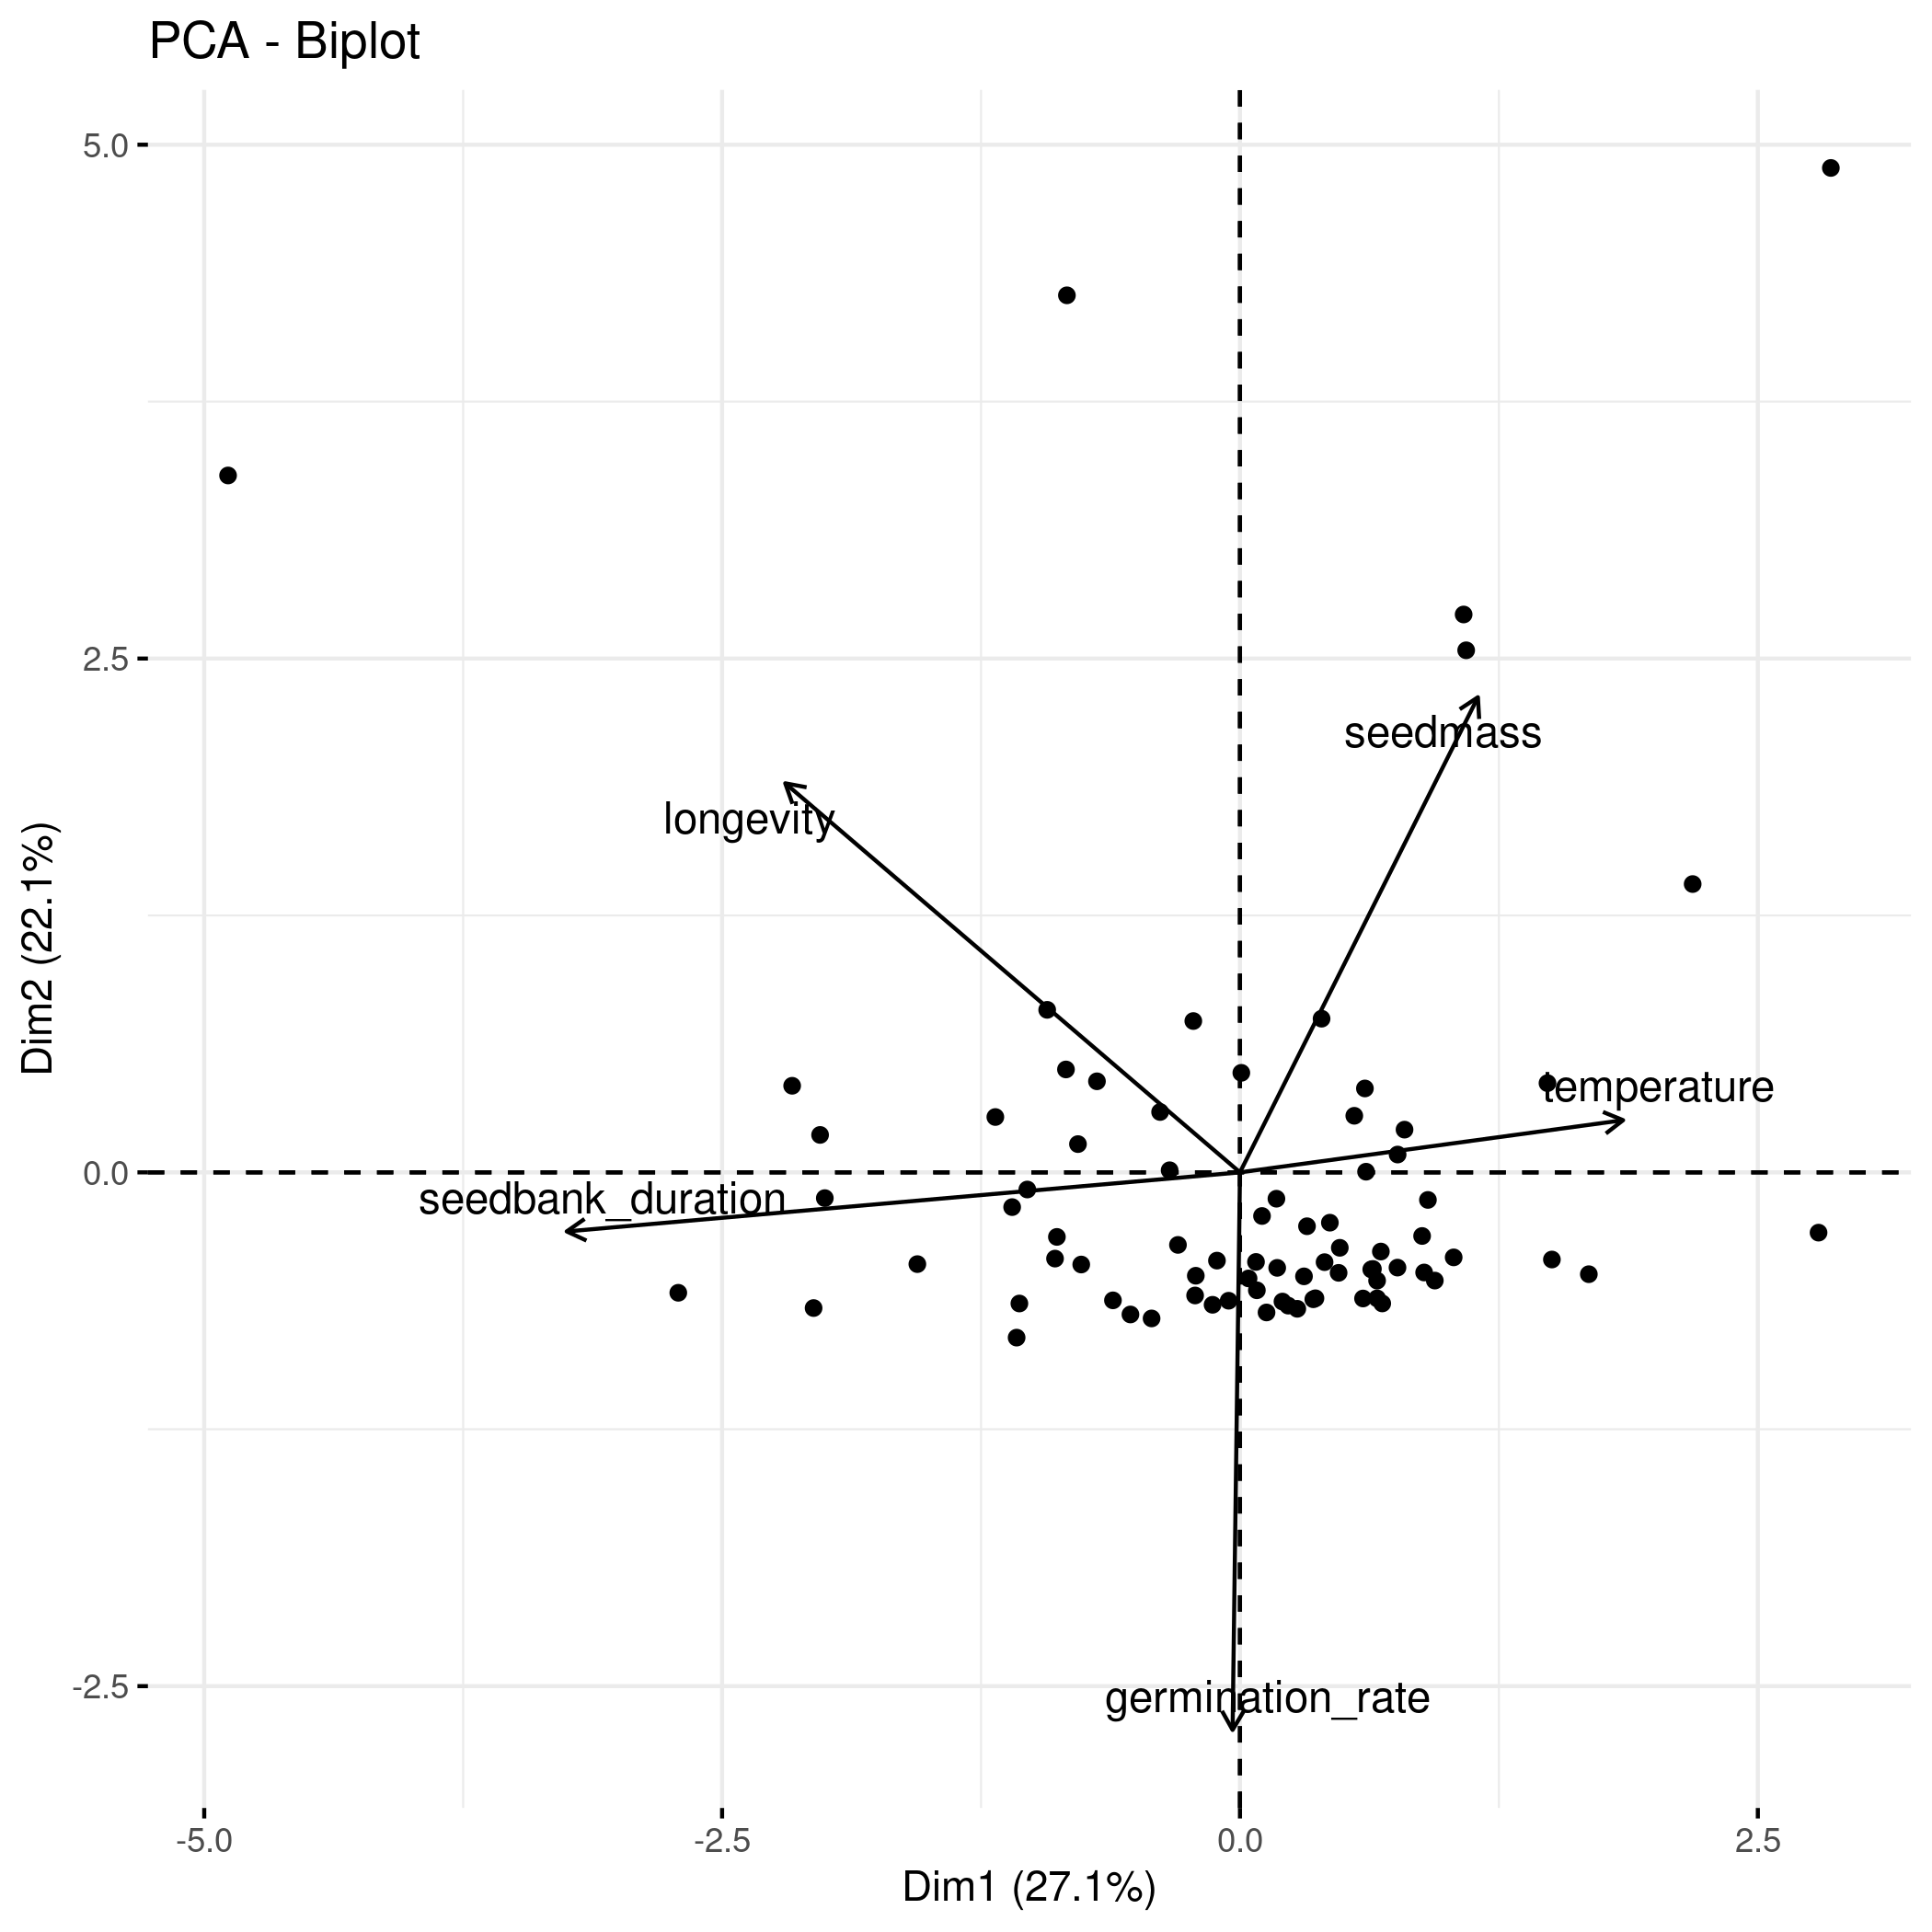
\includegraphics[width= \textwidth]{../result/plot/pca_plot.png}}
        \caption{PCA of traits, we basically reduced the five seed traits to three components. Seedbank duration and longevity are both negative variables and they aligned well with the first component. Seedmass as well as germination rate are both on the second component axis, with seedmass and germination rate opposing in direction. Temperature is a negative vector which is aligned nicely by the third component.}
      \end{figure*}


    \subsection{Functional trait space}

    To provide a more intuitive picture of the effects of cultivation timing on the functional diversity of the Pound Hill community, we needed to construct functional trait spaces for seeds cultivated in different months. Here I chose to build my functional trait space using the funspace package in R and visualize it \citep{funspace}. To construct the functional trait space, we also need to compute the Community Weighted Mean (CWM) to account for abundance differences among species. Changes in average trait values resulting from environmental selection for some functional traits can be well quantified by the Community Weighted Mean (CWM) \citep{ricotta2011cwm}. Because CWM corresponds to the mean of each trait in the community weighted by the relative abundance of the respective species, on average, a greater weight implies a greater abundance of species. The formula for CWM is:

      \begin{equation} CWM = \sum_{i=1}^n p_i x_i \end{equation}

    Where $CWM$ is the community-weighted mean of the functional traits, $p_i$ is the relative abundance of species i (i = 1, 2,..., n), and $x_i$ is the trait value for species i. However, we got our cwm directly using the cwm function in the BAT package \citep{BAT}.

    Functional trait space figures were drawn for the whole site and for the communities cultivated in March, May, and October, respectively. We employed eight linear mixed models(by R package lme4) to further explore the impacts of cultivation timing on the functional composition and diversity of the community \citep{lme4}. Our response variables consisted of community-weighted means derived from z-standardized seed traits, including seed mass, longevity, germination rate, germination temperature, and seedbank duration, alongside functional richness, evenness, and divergence. The fixed factor in each linear mixed model was the cultivation month, categorized into three levels: March, May, and October. To address the pseudoreplication of plot measurements across different years and account for variations between blocks, random effects were specified for year and block. All model assumptions were thoroughly evaluated and no instances of assumption violations were identified.

    \subsection{Predictive model}

    The Fourth Corner model can be implemented with the function traitglm in the R package mvabund \citep{mvabund}. I chose the two site variables of year and month as environmental variables, along with species coverage and trait values, to predict species abundance in different years with different cultivation months. To evaluate the fit of the model, I randomly sampled 80\% of the sites and corresponding species abundance as model training data and the remaining 20\% of the data as test data to evaluate the model fitting. Different combinations of traits were tested under the optimal combination of environmental variables to explore the optimal combination of environmental variables and traits that would predict the best outcome. All simulations were repeated 1000 times.

    The two metrics I chose to evaluate the model fitting were Root Mean Square Error (RMSE) and the coefficient of determination (R-squared). The coefficient of determination is the proportion of variation in the dependent variable explained by the predictive model, ranging between 0 and 1, and is used to assess how accurately the statistical model fits the predicted outcomes. The formula for R-squared is:

      \begin{equation} R-squared = (\frac{n\sum x y - (\sum x) (\sum y)}{\sqrt{(n \sum x^2 - (\sum x)^2) (n \sum y^2 - (\sum y)^2)}})^2 \end{equation}

    Where $x$ is the real value, $y$ is the predicted value, and $n$ is the simple size.


    \section{Results}

    \subsection{Relative abundance}
    
    In October, March, and May, the mean total abundance of species after cultivation was 166.235, 160.190, and 128.765, respectively. The top five most abundant species after October cultivation were Holcus mollis, Agrostis gigantea, Vulpia myuros, Rumex acetosella, and Bromus hordeaceus, with relative abundances of 0.414, 0.109, 0.096, 0.056, and 0.044, respectively. In March, they were Artemisia vulgaris, Fallopia convolvulus, Agrostis gigantea, Achillea millefolium, and Holcus mollis, with relative abundances of 0.349, 0.099, 0.092, 0.076, and 0.072, respectively. In May, they were Erodium cicutarium, Spergula arvensis, Bromus sterilis, Agrostis gigantea, and Chenopodium album, with relative abundances of 0.273, 0.201, 0.086, 0.071, and 0.069, respectively.

    \subsection{Functional diversity and functional trait space}
      
    From Figure 2, we can see that the red areas were not biased towards any trait, which suggested that the probability distribution of traits was relatively centralised and density was highest in the center of the space. Next, we will explore the funspace grouped by month of cultivation.

      \begin{figure}[H]
        \centering
        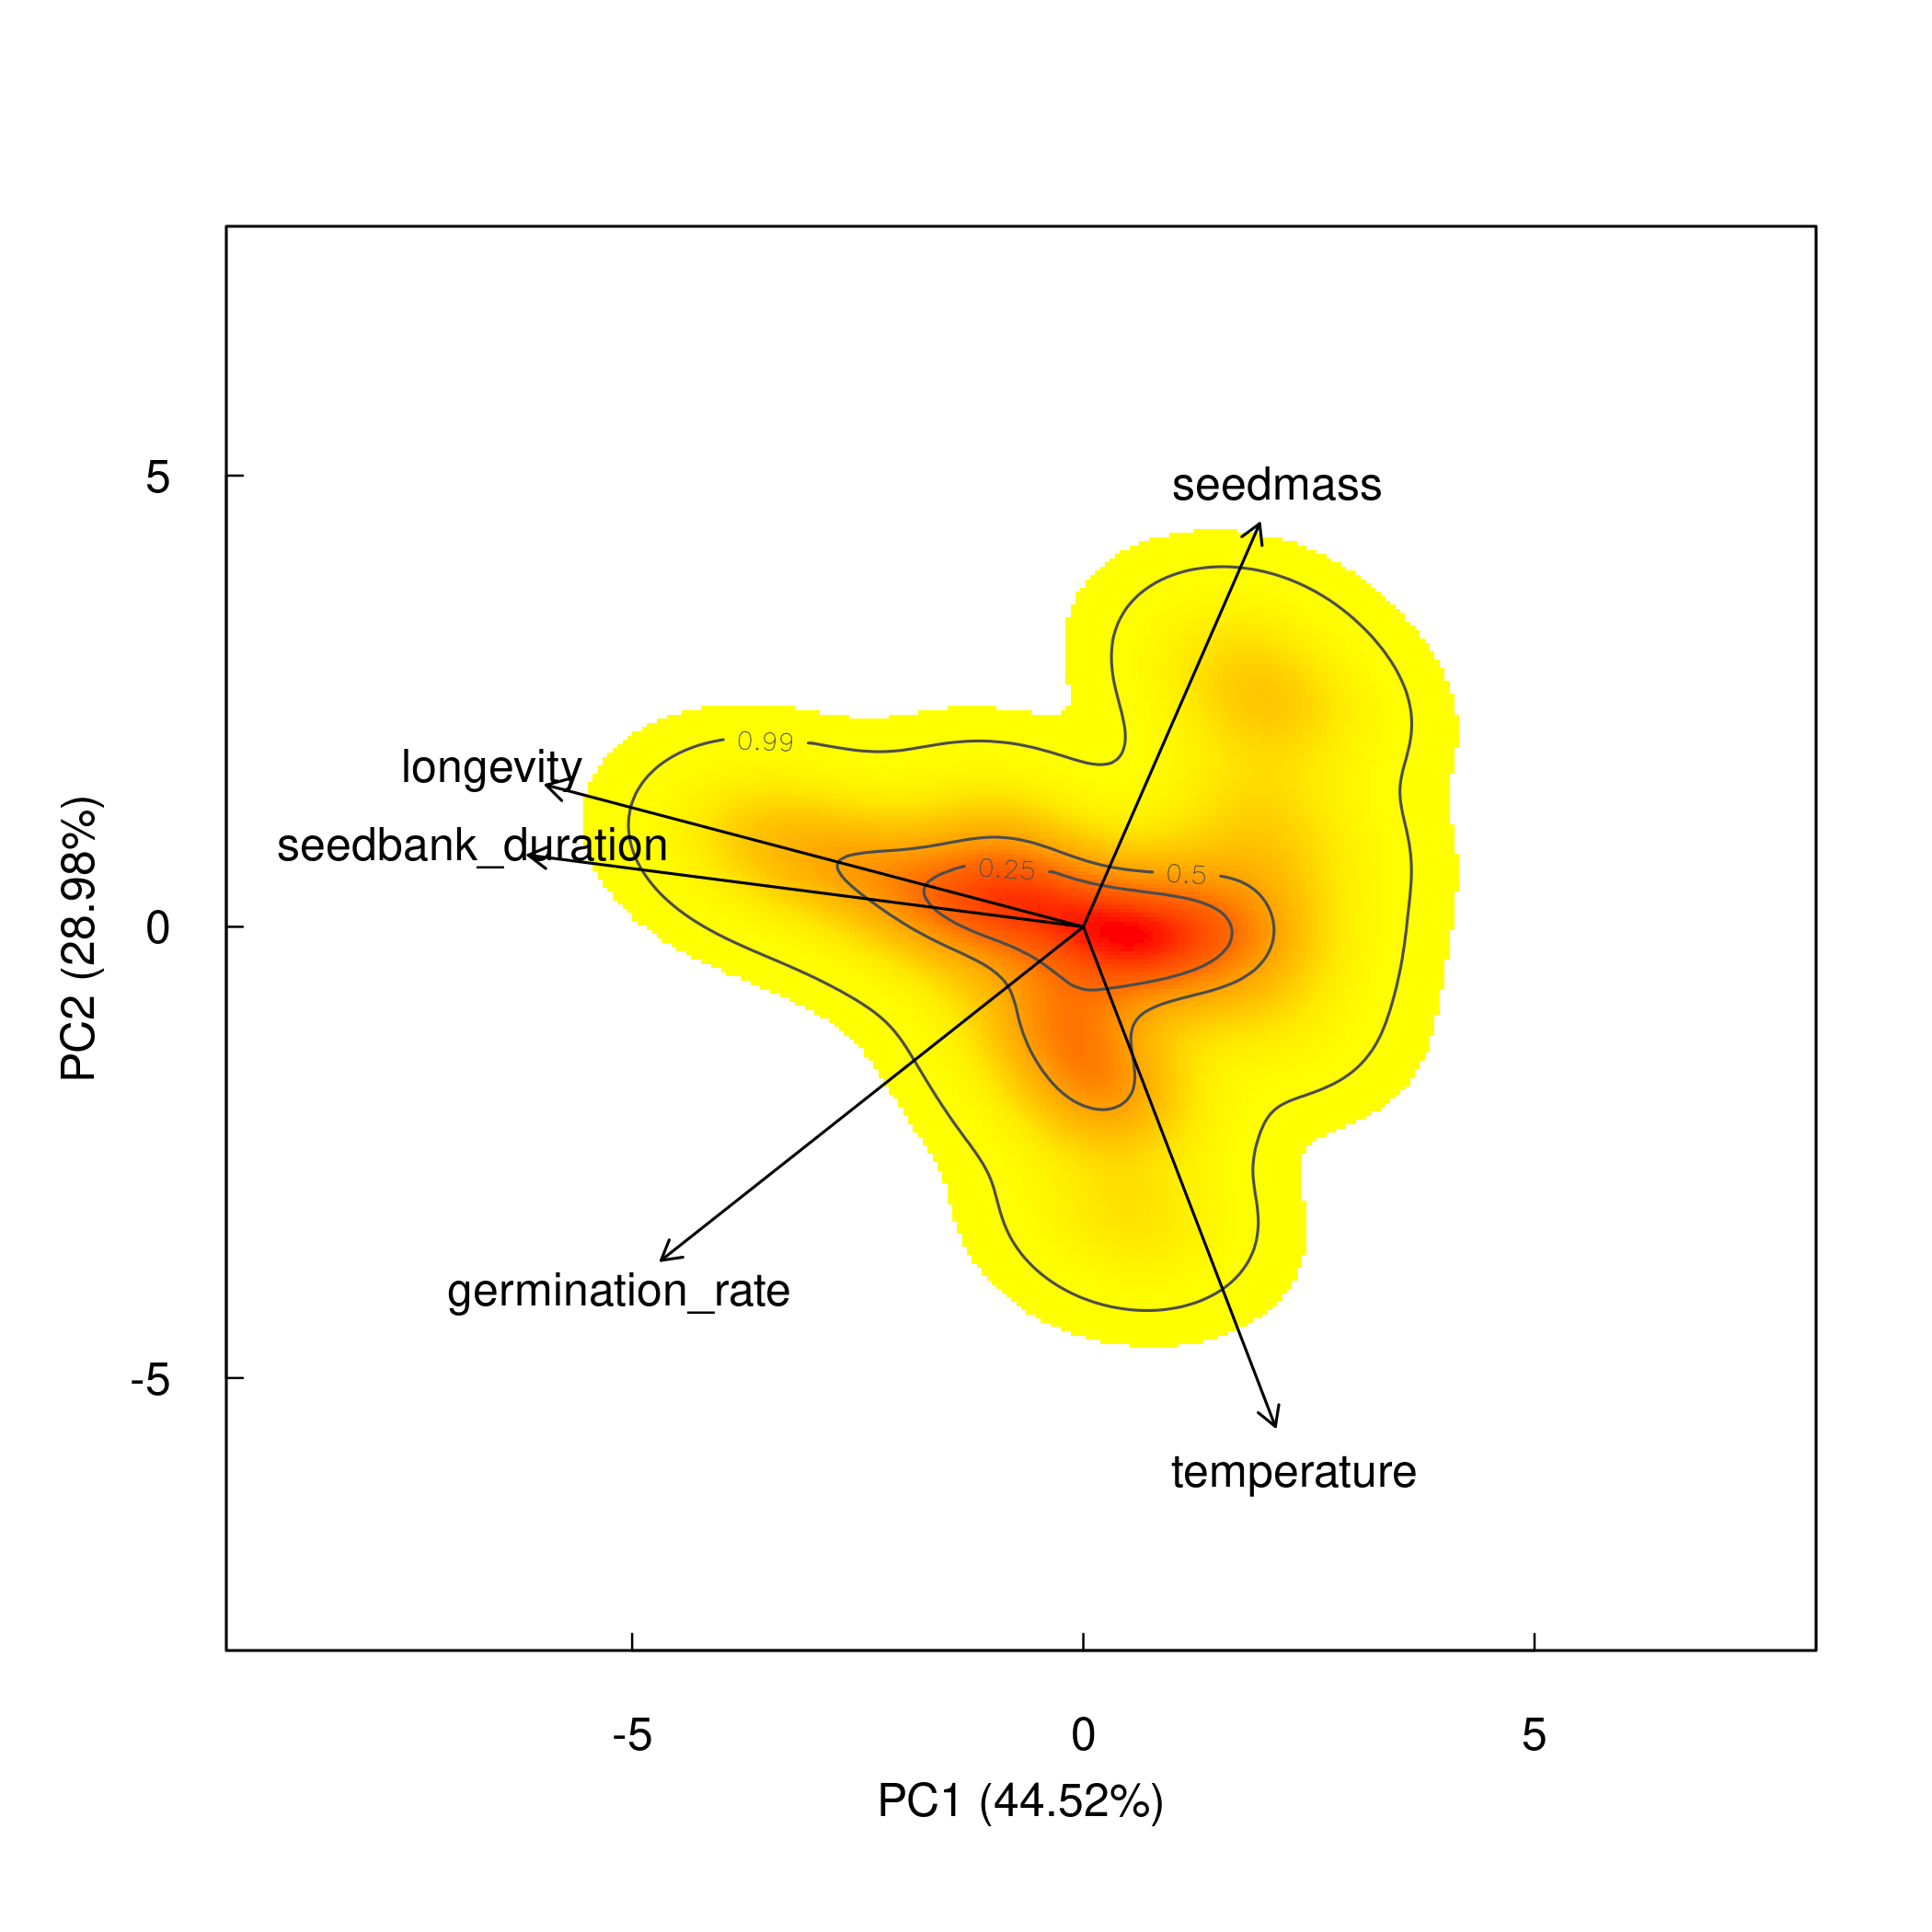
\includegraphics[width=0.8\textwidth]{../result/plot/traitspace_global.png}
        \caption{A global funspace plot created by the function funspace(), with the 0.99, 0.5, and 0.25 quartiles of the probability distribution represented by contour lines. The probability distributions of traits in the functional trait space defined by PCA are represented by different colors, where red represents a high probability and yellow a low probability.}
      \end{figure}

    From Figure 3, the high-probability region was distributed between germination rate and germination temperature in March. In May, the high-probability region was distributed in the direction of seed longevity and seedbank duration, followed by germination rate. In October, the high-probability region was more biased in the direction of seedmass. This suggests that March is characterised by species with a warmer seed germination temperature; May by species with greater seedbank duration and October by larger seed species.

      \begin{figure}[H]
        \centering
        \makebox[1 \textwidth][c]{
        \resizebox{1.4 \textwidth}{!}{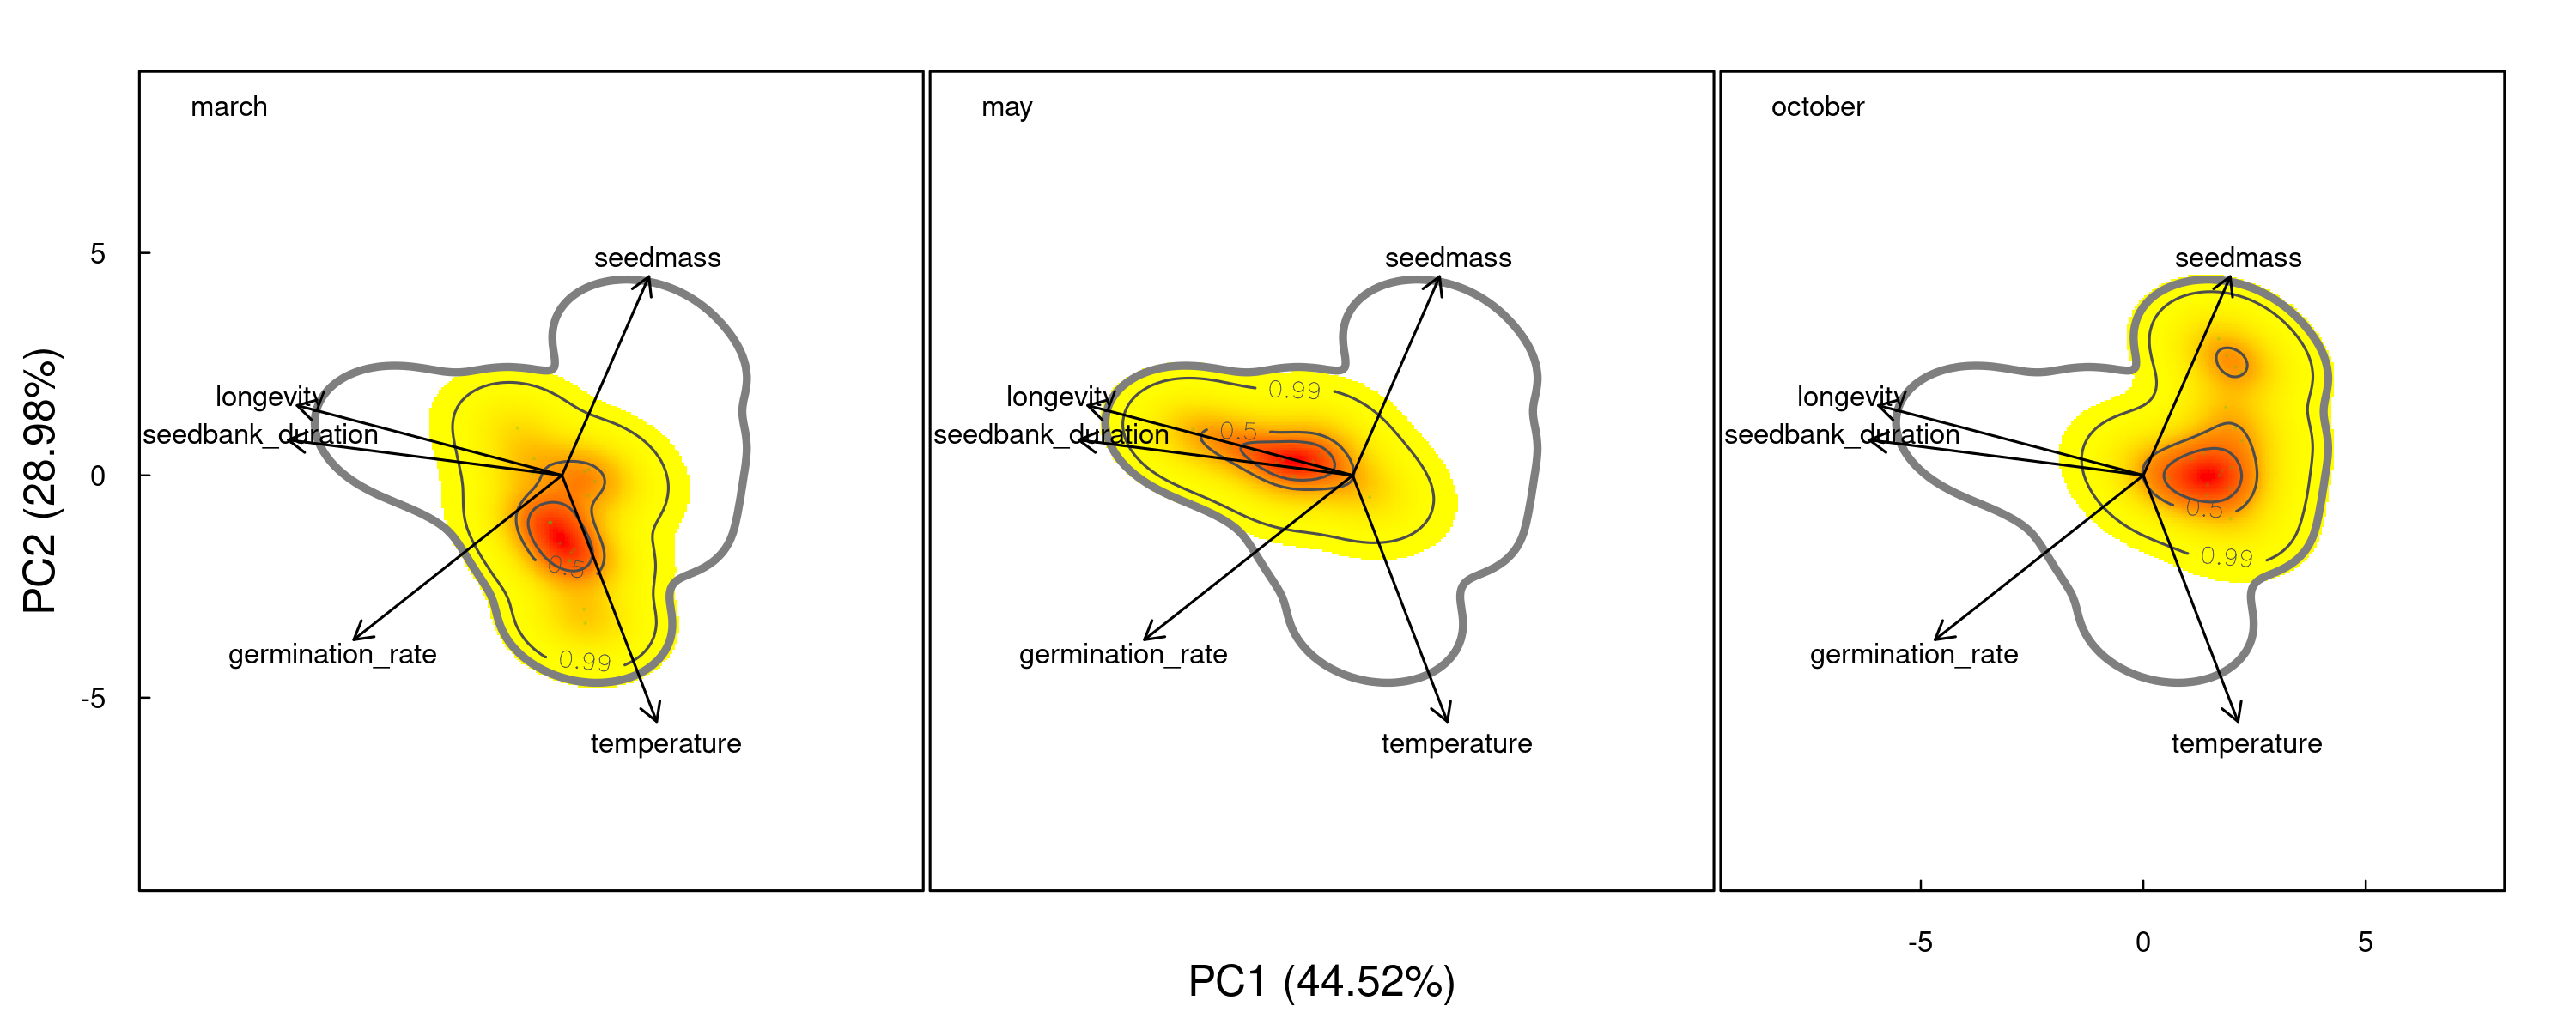
\includegraphics{../result/plot/traitspace_groups.png}}}
        \caption{A funspace plot created with the function funspace() is grouped by month of cultivation, including groups for the three months of cultivation (March, May, and June). The same as in Figure 2: the 0.99, 0.5, and 0.25 quartiles of the probability distribution are represented by the contour lines. The probability distributions of traits in the functional trait space defined by PCA are represented by different colors, where red represents a high probability and yellow a low probability.}
      \end{figure}

      \begin{table}[H]
        \begin{center}
          \label{tab:table1}
          \makebox[1 \textwidth][c]{
            \resizebox{1.35 \textwidth}{!}{
            \begin{tabular}{||c c c c c c||} 
            \textbf{} & \textbf{Seed mass} & \textbf{Seed longevity} & \textbf{Germination rate} & \textbf{Germination temperature} & \textbf{Seedbank duration}\\
            \hline
            Fixed Effects CI and Mean\\
            March & (-0.159, -0.155, -0.151) & (-0.425, 0.0186, 0.462) & (0.2014, 0.28197, 0.3625) & (0.3635, 0.555, 0.7464) & (-0.156, 0.132, 0.419) \\
            May & (-0.158, -0.154, -0.150) & (1.008, 1.4517, 1.895) & (0.2320, 0.31250, 0.3930) & (-0.3069, -0.115, 0.0761) & (0.195, 0.483, 0.770) \\
            October & (-0.155, -0.151, -0.147) & (-0.772, -0.3285, 0.115) & (-0.0894, -0.00887, 0.0717) & (-0.0769, 0.115, 0.3060) & (-0.691, -0.404, -0.117) \\
            \\
            Random Effects Variance \\
            Year & 8.419e-06 & 0.07459 & 0.002568 & 0.01726 & 0.04984 \\
            Block & 0.000e+00 & 0.00000 & 0.001168 & 2.632e-20 & 1.705e-10 \\
            Residual & 2.102e-05 & 0.52536 & 0.009248 & 0.07522 & 0.07584 \\
            \\
            Conditional and marginal R-squared \\
            R2m & 0.09120972 & 0.5015914 & 0.6216614 & 0.4596377 & 0.5181713\\
            R2c & 0.351082 & 0.5635576 & 0.7305209 & 0.5604812 & 0.7092461 \\
          \end{tabular}
          }
          }
          \caption{Results of the CWMs linear mixed model: For fixed effects, the 95\% confidence intervals for the CWMs for each cultivation month are shown. Where the numbers in the middle of the brackets are the mean, and the lower and upper bounds of the confidence intervals are shown on the left and right sides. For random effects, the variances of year, block, and residual are shown. For Conditional and marginal R-squared, they represent the variance explained by the entire model (both fixed and random factors) and the fixed factor, respectively. Where $R2m$ denotes marginal R-squared, $R2c$ denotes conditional R-squared.}
        \end{center}
      \end{table}

      Five linear mixed models (refer to Table 1 and Figure 4) found the following trends: Seed mass slightly increased in plant communities cultivated in October, while seed longevity significantly increased in May. The germination rates were significantly higher in both March and May cultivations. March cultivation was linked to a discernible rise in germination temperature, whereas May cultivation notably prolonged the seedbank duration. The cultivation month explained variability in seed traits ranging from 9.12\% to 62.17\%. While random effects, particularly year, accounted for 6.20\% to 25.99\%. Among these effects, disparities between years exerted the most substantial impact on seedbank duration and the least on seed longevity. This means that the seedbank duration varies significantly across different years, while the variation in seed longevity remains relatively small.


      \begin{table}[H]
        \begin{center}
          \label{tab:table1}
          \resizebox{1 \textwidth}{!}{
            \begin{tabular}{||c c c c||}
            \textbf{} & \textbf{FRic} & \textbf{FEve} & \textbf{FDiv}\\
            \hline
            Fixed Effects CI and Mean\\
            March & (0.248, 4.29, 8.34) & (0.318, 0.419, 0.520) & (0.738, 0.798, 0.858) \\
            May   & (4.355, 8.40, 12.44) & (0.407, 0.508, 0.609) & (0.667, 0.728, 0.788) \\
            October & (3.455, 7.50, 11.54) & (0.261, 0.362, 0.463) & (0.526, 0.586, 0.646) \\
            \\
            Random Effects Variance \\
            Year  & 10.2087  & 0.00583  & 5.745e-04  \\
            Block & 0.3365  & 0.00000  & 9.933e-18  \\
            Residual & 10.0535 & 0.01257 & 1.420e-02 \\
            \\
            Conditional and marginal R-squared \\
            R2m & 0.1329805 & 0.1662398 & 0.3495998 \\
            R2c & 0.5768396 & 0.4304188 & 0.3748981 \\
          \end{tabular}
          }
          \caption{Results of the functional diversity metrics(FRic, Feve, and FDiv) linear mixed model: For fixed effects, the 95\% confidence intervals for the functional diversity metrics for each cultivation month are shown. Where the numbers in the middle of the brackets are the mean, and the lower and upper bounds of the confidence intervals are shown on the left and right sides. For random effects, the variances of year, block, and residual are shown. For Conditional and marginal R-squared, they represent the variance explained by the entire model (both fixed and random factors) and the fixed factor, respectively. Where $R2m$ denotes marginal R-squared, $R2c$ denotes conditional R-squared.}
        \end{center}
      \end{table}

    Three linear mixed models (refer to Table 2 and Figure 4) revealed distinct patterns: functional richness exhibited significant increases in communities cultivated during May and October, functional evenness was notably higher in May, and higher functional divergence was observed in March and May. On the other hand, cultivating in October resulted in less functionally diverse plant communities. The cultivation month was found to explain 13.30\% to 34.96\% of the variance in the functional diversity indices. While random effects, particularly year, accounted for 2.52\% to 44.39\%. Among these effects, differences between years played the most substantial role in influencing functional richness and had the least impact on functional divergence. This suggests that the occupancy of the seed functional space varies significantly from year to year, while the dispersion in the seed trait space remains relatively consistent. However, cultivation timing predominantly affects the divergence within the seed trait space.


      \begin{figure}[H]
        \centering
        \makebox[0.8 \textwidth][c]{\resizebox{1 \textwidth}{!}{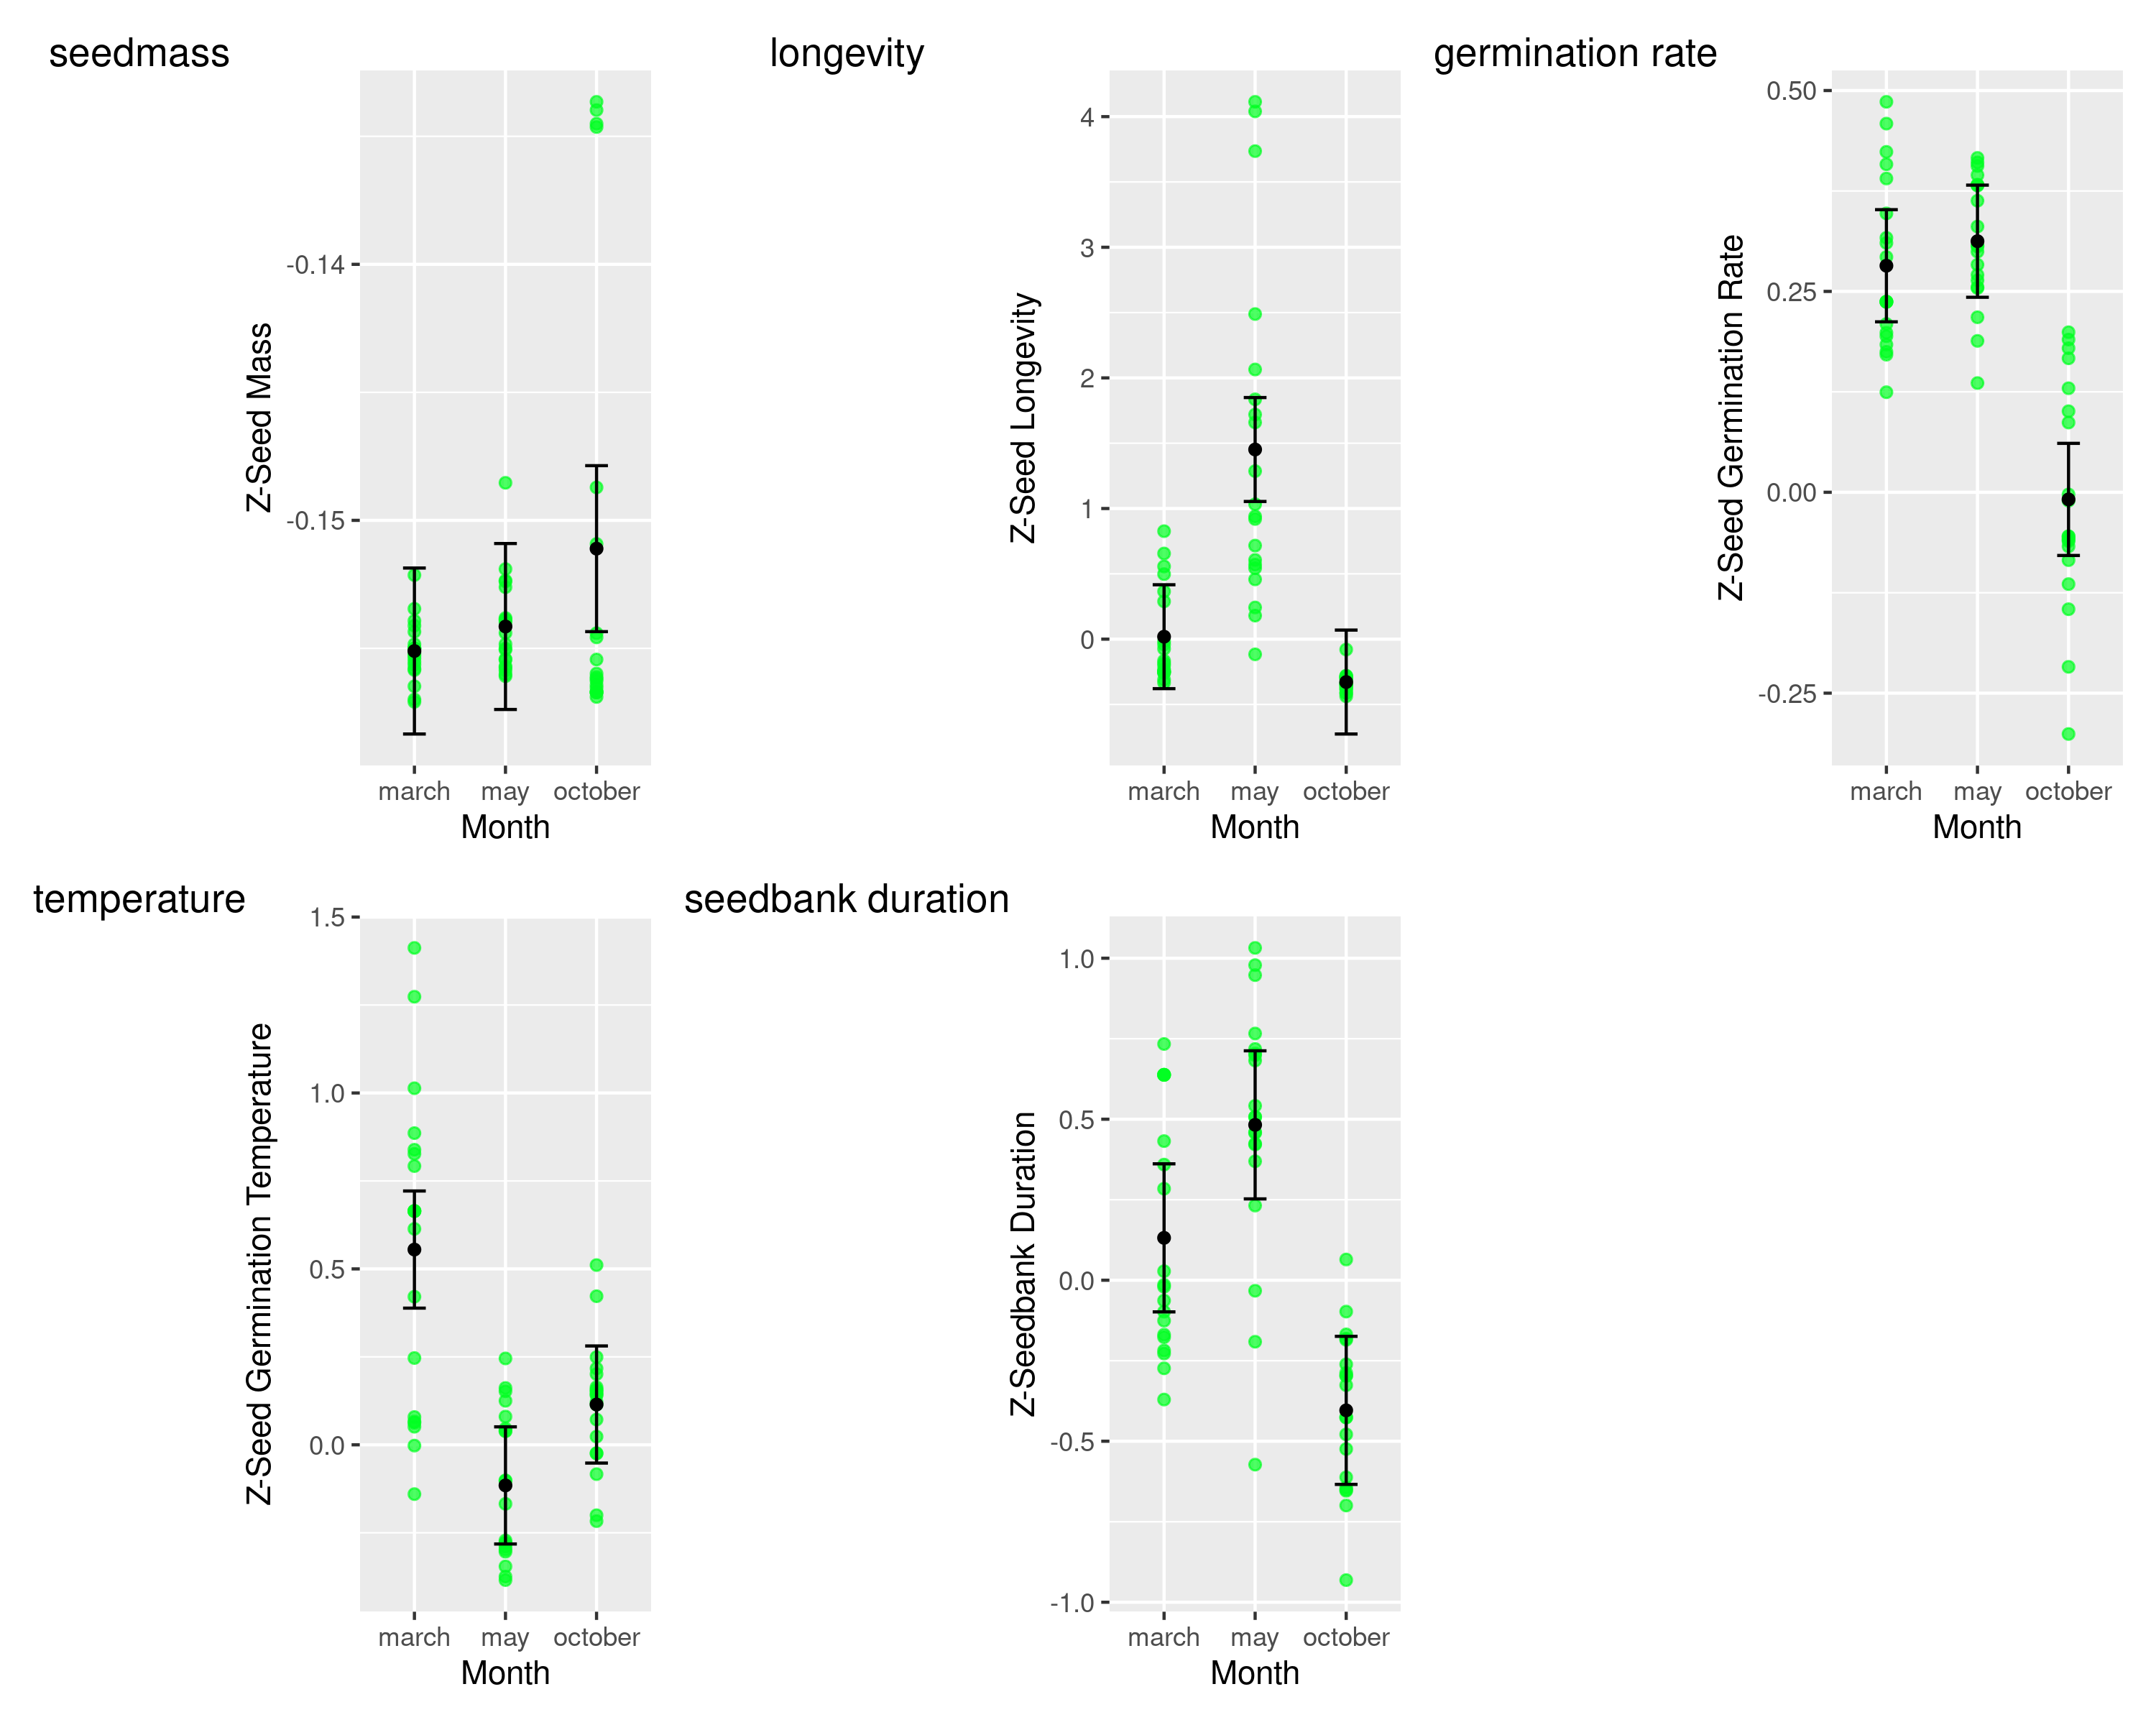
\includegraphics{../result/plot/emmeans_traits.png}}}
        \makebox[0.8 \textwidth][c]{\resizebox{1 \textwidth}{!}{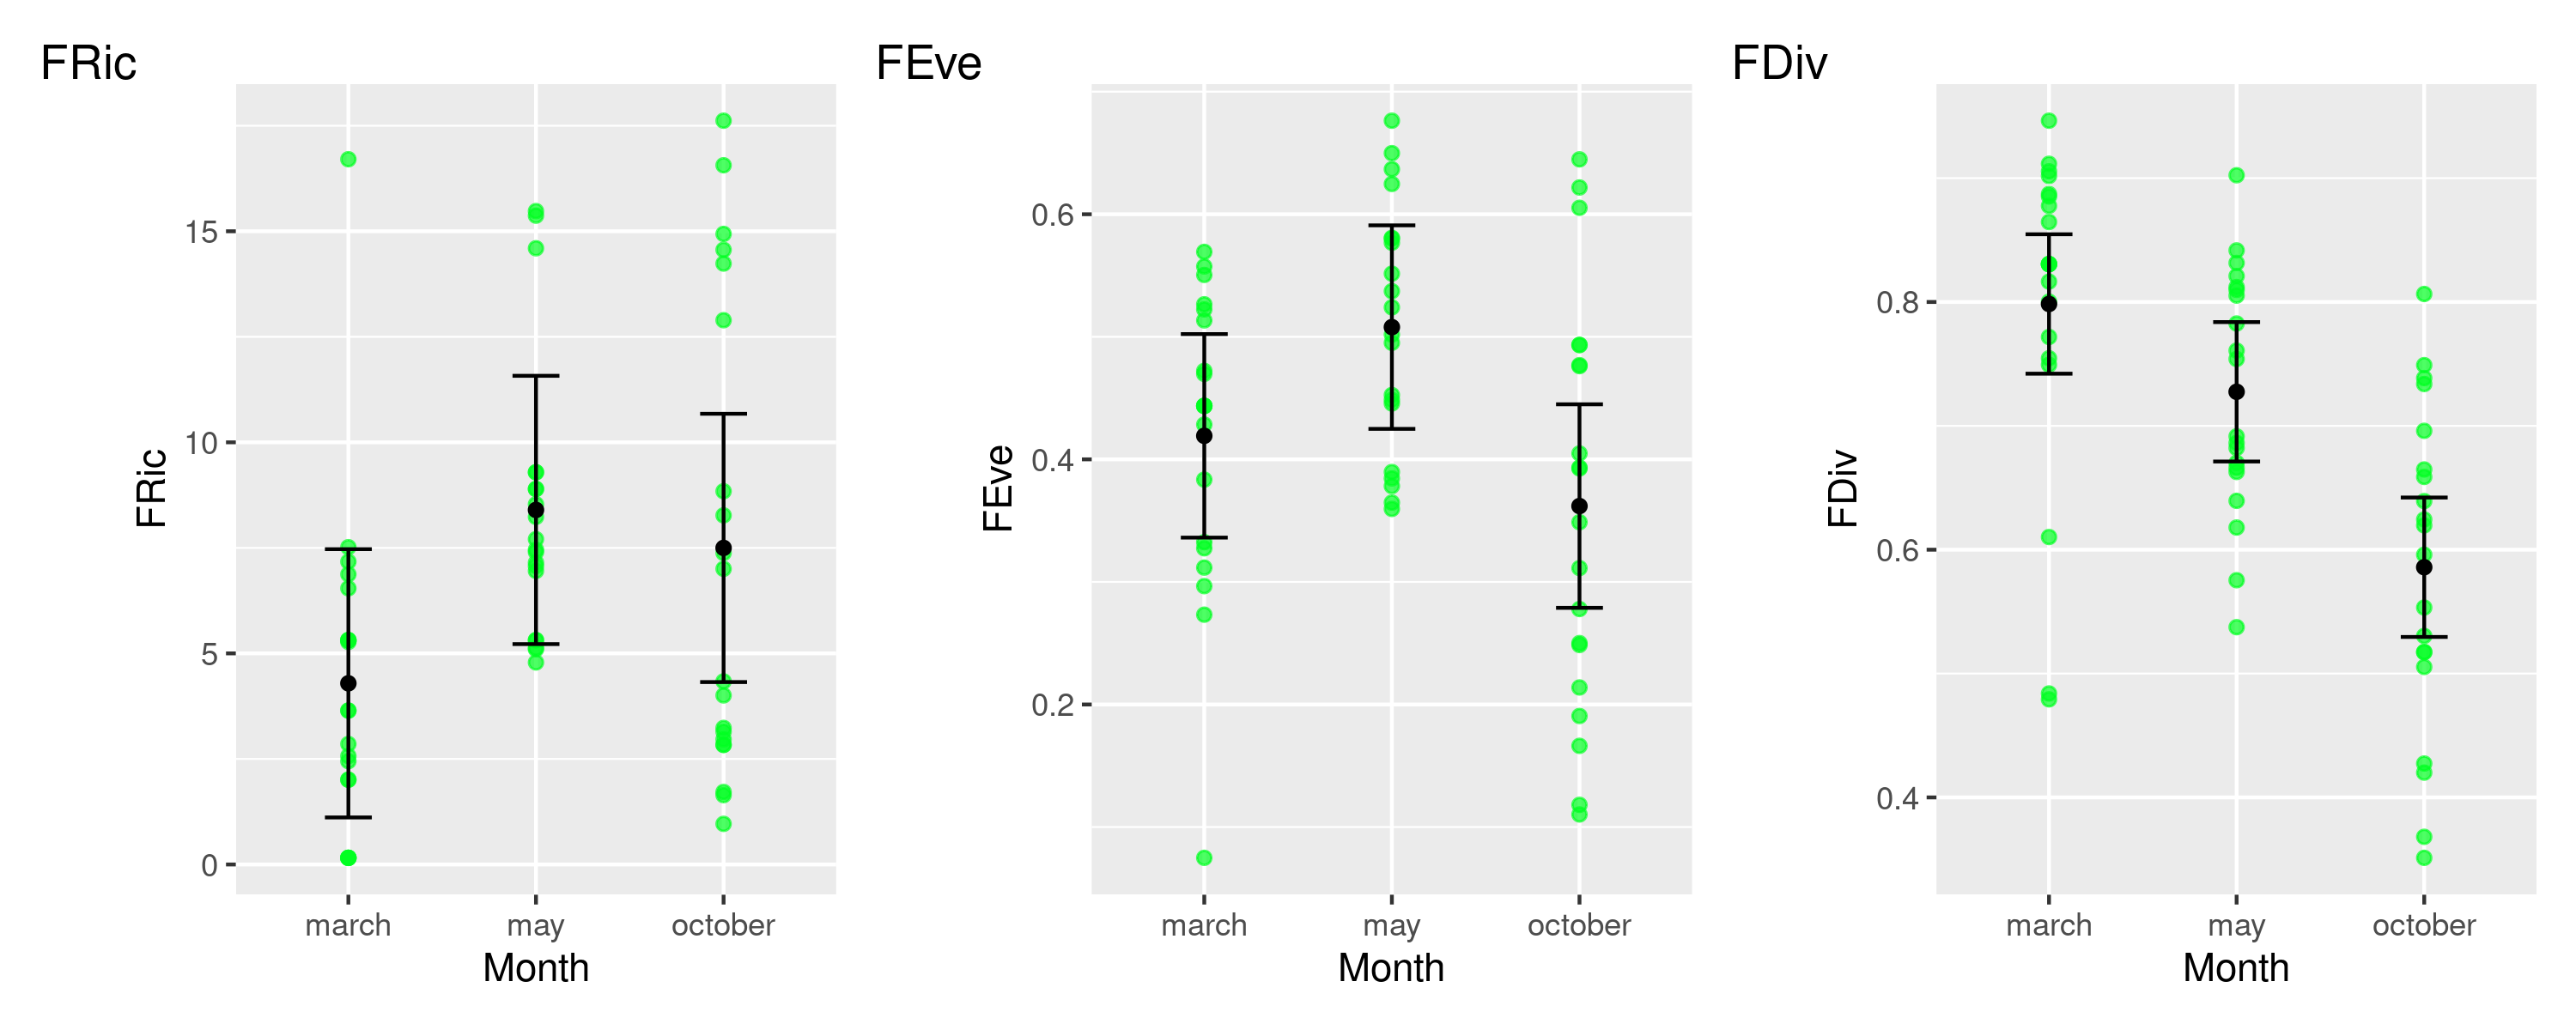
\includegraphics{../result/plot/emmeans_metrics.png}}}
        \caption{Plots of estimated marginal means results for five traits and three functional diversity metrics after cultivation in March, May and October, respectively. The black dots indicate the corresponding estimated marginal means and the lines though dots indicate the corresponding 95\% confidence intervals. Green dots indicate the real values of the z-standardized trait CWMs and functional diversity metrics.}
      \end{figure}
      

      \subsection{Relative abundance prediction}
 
    From Table 3, we could see that using two environmental variables predicted more accurately than using three environmental variables when all traits were used. Month\&Plot and Year\&Month as the two groups with the smaller RMSE values, were fairly close to each other. However, the Year\&Month group had the maximal R-squared value among all the groups; hence, the Year\&Month group will be used as the optimal environmental variable group to explore the best combination of traits under the optimal environmental variables.


       \begin{table}[H]
        \begin{center}
          \makebox[0.8 \textwidth][c]{
          \resizebox{1.2 \textwidth}{!}{
            \begin{tabular}{||c c c c c||} 
            \textbf{} & \textbf{R-squared confidence interval} & \textbf{R-squared mean} & \textbf{RMSE confidence interval} & \textbf{RMSE mean} \\
            \hline
            Month\&Plot                  & (0.2576767, 0.270784) & 0.2642304 & (0.00956456, 0.009704401) & 0.00963448 \\
            \\
            Year\&Plot                   & (0.1620703, 0.17462) & 0.1683451 & (-205.0268, 747.5673) & 271.2702 \\
            \\
            Year\&Month                  & (0.3153804, 0.3301238) & 0.3227521 & (0.009665446, 0.01041586) & 0.01004065 \\
            \\
            All environmental variables  & (0.1620834, 0.174631) & 0.1683572 & (-205.4695, 749.0831) & 271.8068 \\
          \end{tabular}
          }
          }
          \caption{Metrics(Means and 95\% confidence intervals for R-squared and RMSE) for assessing the predictions of the Traitglm model when using all traits with Month\&Plot, Year\&Plot, Year\&Month, and All environmental variables(Year, Month, and Plot) as inputs to the environmental variables, respectively.}
        \end{center}
      \end{table}
      
      The predictive impacts of Year and Month were evaluated upon inclusion as environmental variables. As depicted in Table 4, the RMSE values experienced a substantial reduction as the count of traits increased. When transitioning from 1 to 2 traits, there was a noteworthy escalation in the R-squared value; however, as the trait count continued to rise, the alteration in the R-squared value became marginal. The two optimal trait combinations were longevity and seedbank duration, and longevity, seedbank duration, and seedmass. Their R-squared values ranged from 0.351 to 0.366 which were still weak, suggesting that even these optimal combinations do not make ideal predictions.

      \begin{table}[H]
        \begin{center}
          \makebox[1 \textwidth][c]{
          \resizebox{1.2 \textwidth}{!}{
            \begin{tabular}{||c c c c c||} 
            \textbf{} & \textbf{R-squared confidence interval} & \textbf{R-squared mean} & \textbf{RMSE confidence interval} & \textbf{RMSE mean} \\
            \hline
            Single trait group \\
            sm      & (0.0005941327, 0.0007720451) & 0.0006830889 & (0.009437903, 0.009567967) & 0.009502935 \\
            l       & (0.04565699, 0.05181713) & 0.04873706 & (-2.979263e+101, 1.846779e+102) & 7.744263e+101 \\
            gr      & (8.306026e-05, 8.930851e-05) & 8.618439e-05 & (-5.067871e+56  8.217612e+57) & 3.855412e+57 \\
            t       & (0.001841745, 0.004228039) & 0.003034892 & (-384387939, 1587094615) & 601353338 \\
            sd      & (0.0001289644, 0.0006991556) & 0.00041406 & (1.186047e+17, 8.572677e+18) & 4.345641e+18 \\
            \\
            Two traits group \\
            sm\&l      & (0.2987876, 0.3114917) & 0.3051397 & (-1183441332, 7301151455) & 3058855061 \\
            sm\&gr     & (0.2803984, 0.2932514) & 0.2868249 & (-1.436498e+14, 2.488271e+15) & 1.17231e+15 \\
            sm\&t      & (0.2645367, 0.2760386) & 0.2702876 & (-0.06186653, 0.2300023) & 0.08406789 \\
            sm\&sd     & (0.3404088, 0.3550468) & 0.3477278 & (0.01031783, 0.02420642) & 0.01726213 \\
            l\&gr      & (0.2830908, 0.2962891) & 0.28969 & (-376274.3, 6366739) & 2995232 \\
            l\&t       & (0.3334936, 0.3480077) & 0.3407506 & (-2.422486, 7.502623) & 2.540069 \\
            l\&sd      & (0.3511552, 0.3658807) & 0.3585179 & (0.00966004, 0.00998687) & 0.009823455 \\
            gr\&t      & (0.3184528, 0.3328823) & 0.3256676 & (-2.454107, 8.472298) & 3.009095 \\
            gr\&sd     & (0.3347589, 0.3495199) & 0.3421394 & (-1.867611e+19, 5.749001e+19) & 1.940695e+19 \\
            t\&sd      & (0.3178401, 0.332375) & 0.3251076 & (0.009605426, 0.00979318) & 0.009699303 \\   
            \\
            Three traits group \\
            sm\&l\&gr    & (0.2831884, 0.2963898) & 0.2897891 & (-402090.7, 6813022) & 3205466 \\
            sm\&l\&t     & (0.3334691, 0.3479841) & 0.3407266 & (-2.56789, 7.950081) & 2.691095 \\
            sm\&l\&sd    & (0.351444, 0.3661143) & 0.3587791 & (0.009678934, 0.0099895) & 0.009834217 \\
            sm\&gr\&t    & (0.3184187, 0.3328498) & 0.3256342 & (-2.333605, 7.986831) & 2.826613 \\
            sm\&gr\&sd   & (0.3344556, 0.3492233) & 0.3418394 & (-4.39061e+19, 1.351546e+20) & 4.562425e+19 \\
            sm\&t\&sd    & (0.3177729, 0.3323071) & 0.32504 & (0.009604238, 0.009792618) & 0.009698428 \\
            l\&gr\&t     & (0.3156718, 0.3304521) & 0.323062 & (-1.79154, 36.81389) & 17.51118 \\
            l\&gr\&sd    & (0.3229128, 0.3373526) & 0.3301327 & (0.009589555, 0.009774876) & 0.009682215 \\
            l\&t\&sd     & (0.3172593, 0.3318523) & 0.3245558 & (0.009606746, 0.009794833) & 0.009700789 \\
            gr\&t\&sd       & (0.3160232, 0.3306593) & 0.3233413 & (0.004382345, 0.1689851) & 0.08668373 \\   
            \\     
            Four traits group \\
            sm\&l\&gr\&t  & (0.3156607, 0.3304412) & 0.3230509 & (-1.940306, 39.76386) & 18.91178 \\
            sm\&l\&gr\&sd & (0.3228455, 0.337286) & 0.3300658 & (0.009588829, 0.009774601) & 0.009681715 \\
            sm\&l\&t\&sd  & (0.3172038, 0.3317977) & 0.3245007 & (0.009608636, 0.009796445) & 0.009702541 \\
            sm\&gr\&t\&sd & (0.316, 0.3306359) & 0.323318 & (0.005979528, 0.1247685) & 0.06537404 \\
            l\&gr\&t\&sd  & (0.3153961, 0.3301434) & 0.3227697 & (0.009653782, 0.01118025) & 0.01041702 \\
            \\
            Five traits group \\
            all        & (0.3153804, 0.3301238) & 0.3227521 & (0.009665446, 0.01041586) & 0.01004065 \\
          \end{tabular}
          }
          }
          \caption{Assessment of the metrics(Means and 95\% confidence intervals for R-squared and RMSE) for predictions of the Traitglm model using different combinations of traits when only Year and Month are used as inputs for environmental variables. Where $sm$ denotes seedmass, $l$ denotes longevity, $gr$ denotes germination rate, $t$ denotes temperature, and $sd$ denotes seedbank duration.}
        \end{center}
      \end{table}


    \section{Discussion}
    
    We found that cultivation timing did have a significant effect on the functional trait composition and diversity of species. The number of traits in the Fourth Corner model and the choice of environmental variables affected the abundance prediction, with more traits potentially improving the accuracy of predictions and the explainability of the model, whereas the inclusion of cultivated plots as an environmental variable might not have been as effective.

    Cultivation in March resulted in Pound Hill plants having seeds with high germination rates and the highest germination temperatures, whilst having a greater functional divergence, which could mean intense competition for functionally similar species among the communities cultivated in March \citep{mammola2021concepts, jimenez2016seed}. In contrast, species in Pound Hill had the highest functional richness and evenness after May cultivation, and their seeds had the highest germination rates as well as the longest seed longevity and seed bank duration. Pound Hill communities cultivated in May were more even in resource utilization, with seed persistence dispersing risk and being more resistant to invaders \citep{saatkamp2019research, mason2005functional}. Plants in Pound Hill after October cultivation had larger seed mass, but lower functional evenness and divergence. This suggests that in Pound Hill's plant community cultivated in October, there might be dominant species present, higher functional overlap, lower interspecies competition, and lower resource utilization efficiency. The community structure is simpler, and its resistance to invaders is weaker \citep{mammola2021concepts}. It's worth mentioning that cultivation in March led to higher average germination temperatures for the community's seeds. In March, the prevailing species was Artemisia vulgaris, a frost-resistant plant with an average seed germination temperature of approximately 25.3°C. This temperature was higher compared to the 18.9°C of the dominant species in October (Holcus mollis), as well as the 17.3-19.1°C range for the dominant species in May (Erodium cicutarium and Spergula arvensis). This might suggest that the mean seed germination temperature might not provide insight into the frost resistance at the community level. The growing environment for seedlings varies noticeably: March was relatively cold and humid, while October and May were relatively warm, with October being humid and May comparatively dry. Cultivation in March or October could potentially eliminate frost-sensitive seedlings, but May cultivation would not \citep{crawley2021rise}. Therefore, we infer that the warm and dry conditions in May provided the Pound Hill community with more evenly distributed and favorable resource utilization \citep{saatkamp2019research,mason2005functional}. On the other hand, October cultivation favored species that experienced rapid growth in the second year's spring after enduring a harsh winter \citep{crawley2004timing}, leading to a more pronounced species dominance but simpler community structure \citep{mammola2021concepts}. A simpler community structure might have resulted in the demise of all October germinated species' seedlings after cultivation in March \citep{crawley2004timing}. In contrast, March cultivation benefited from favorable soil moisture conditions, promoting rapid growth of the vernalized seeds' seedlings \citep{crawley2004timing}, potentially causing intense competition among functionally similar species \citep{mammola2021concepts,jimenez2016seed}. The contribution of block to the variability in functional traits and diversity is limited, suggesting that changes in cultivation blocks had minimal influence on functional composition and diversity. Conversely, year accounted for a greater proportion of variation in functional traits and diversity. The timing of cultivation emerged as a primary driver of variation in functional composition and diversity. Building upon the foundation laid by \citet{crawley2004timing,crawley2021rise}, we further assessed the impact of cultivation timing on the functional composition and diversity of the Pound Hill plant community. This aims to provide a more comprehensive understanding of how disturbance timing might influence plant communities. Nevertheless, the absence of detailed environmental data in the context of the Pound Hill Disturbance Experiment prevents us from further assessing the influence of specific environmental conditions on the functional composition and diversity of plant communities. In the future, gathering more detailed environmental data, such as precipitation, temperature, humidity, and soil pH, could be crucial for evaluating the impact of environmental filters on the functional composition and diversity of the plant community.

    In the Fourth Corner model prediction of abundance, it could be seen that the model predicted better when we reduced the number of environmental variables, and the best prediction was achieved when only the year and the month were included as environmental variables in the model. Due to the interaction of traits and environments, it is advisable to attempt to include fewer explanatory variables in the Fourth Corner model \citep{brown2014fourth}. The Month\&Plot and Year\&Month groups performed relatively well in prediction accuracy, but  their RMSE values were still on the same magnitude as the mean of the species relative abundance data (0.01282051). Nevertheless, the predictive performance of the Fourth Corner model was indeed improved by adapting the environmental variables. And we found that fitting more traits into the Fourth Corner model did improve the accuracy of relative abundance prediction. However, we shall keep calm because further increasing the number of traits will also increase the interaction terms between traits and environment in the Fourth Corner model. Therefore, explanatory variables should be carefully selected before using the Fourth Corner model to predict the relative abundance of species. Seed traits can be classified into three types: morphological, biophysical, and germination traits \citep{jimenez2016seed}, selecting traits with representative functional significance among different types of seed traits to include in the model might be a worthwhile strategy to try. One morphological trait (seed mass) as well as four germination traits (seed longevity, germination rate, germination temperature, and seedbank duration) were selected for this research, and no biophysical traits were used. The reason is that biophysical traits are probably not sufficiently representative in plant community studies, while germination traits have been underestimated in community studies \citep{jimenez2016seed}. Predictions of species relative abundance using the Fourth Corner model are feasible when we use appropriate explanatory variables, although the results are still not precise enough(The R-squared values of the two best predictions ranged from 0.351 to 0.366). Incorporating more detailed environmental variables such as temperature, humidity, and soil pH values into the model, rather than just site data, might enhance the predictive performance of the model. Regarding the model itself, enhancing the Fourth Corner model by examining the significance of interaction terms would be crucial for enhancing the precision of predictions. \citep{brown2014fourth}.

    \section{Conclusion}

    In conclusion, our study indicated that the functional composition and diversity of grassland communities varied due to cultivation and soil disturbance at different times of the year. The moderate performance of the Fourth Corner model might have been influenced by the incorporation of only site data as environmental variables. Moving forward, our next step involves gathering more detailed environmental data to further investigate the impact of environmental filters on the functional composition and diversity of plant communities. And I believe that the inclusion of more detailed environmental data will also enhance the predictive capabilities of the Fourth Corner model.

    \section{Data and Code Availability}

    All data and codes in this project are available at https://github.com/shiyuan-huang22/CMEECourseWork/tree/master/Project. For further information of code and data, please see README.md.

    \bibliographystyle{apalike}

    \bibliography{ref}
  
  
  
\end{document}




